\section{Quasi-kategorie i podstawy $\infty$-kategorii}\label{cat:sec:quasicategories}

W nerwie kategorii zwykłej para składanych krawędzi wyznacza dokładnie jeden $2$-sympleks, a wyższe sympleksy kodują zgodność składania. W tym rozdziale osłabimy jednoznaczność wypełnień, zachowując ich istnienie. Będziemy korzystać z kategorii sympleksów, operatorów $d_i,s_i$, rogów i lematu Yonedy z rozdziału~\ref{cat:sec:simplicial-sets}.

\subsection{Quasi-kategorie i słabe składanie}

\begin{definicja}[Quasi-kategoria]\label{cat:def:quasicategory}
Quasi-kategorią (w tym rozdziale również $\infty$-kategorią w sensie $(\infty,1)$) nazywamy zbiór symplicjalny $X$, w którym każdy morfizm
\[
 \Lambda^k[n]\longrightarrow X,\qquad n\geq2,\quad 0<k<n,
\]
ma wypełnienie $\Delta[n]\to X$. Funktorem quasi-kategorii nazywamy morfizm zbiorów symplicjalnych pomiędzy nimi. Obiektami są elementy $X_0$, a krawędź $f\in X_1$ o $d_1f=x$, $d_0f=y$ nazywamy morfizmem $f:x\to y$. Krawędzią identycznościową obiektu $x$ jest $s_0x$.
\end{definicja}
Nie żądamy wypełnialności rogów zewnętrznych. Kompleks Kana jest quasi-kategorią, lecz nie odwrotnie: nerw $N([1])$ jest kontrprzykładem (przykład~\ref{cat:ex:nerve-not-kan}). Nerwy wszystkich małych kategorii są quasi-kategoriami na mocy twierdzenia~\ref{cat:thm:nerve-inner-horns}; w nich wypełnienia rogów wewnętrznych są jedyne.

Dla krawędzi $f:x\to y$, $g:y\to z$ róg $\Lambda^1[2]\to X$ o ścianach $d_2=f$, $d_0=g$ istnieje dzięki równości $d_0f=d_1g$ (stwierdzenie~\ref{cat:prop:simplicial-compatible-faces}). Wypełnienie $u\in X_2$ ma trzecią krawędź $h=d_1u:x\to z$. Typ $h$ wynika z relacji $d_1d_1u=d_1d_2u$ i $d_0d_1u=d_0d_0u$. Nazywamy $h$ jednym ze złożeń $g$ z $f$. Nie jest to z góry jednoznaczna operacja na zbiorze krawędzi.

\begin{center}
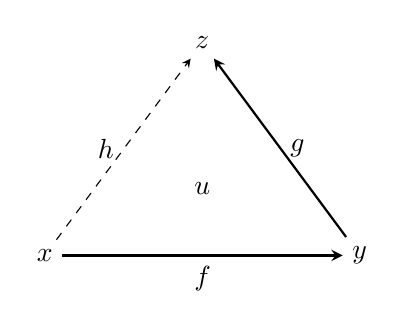
\begin{tikzpicture}[>=stealth]
 \node (x) at (0,0) {$x$};
 \node (y) at (4,0) {$y$};
 \node (z) at (2,2.7) {$z$};
 \draw[->,thick] (x)--node[below] {$f$}(y);
 \draw[->,thick] (y)--node[right] {$g$}(z);
 \draw[->,dashed] (x)--node[left] {$h$}(z);
 \node at (2,.85) {$u$};
\end{tikzpicture}
\end{center}
Linie ciągłe przedstawiają dane rogu, linia przerywana i oznaczenie $u$ -- dane uzyskane przez wybór wypełnienia. W quasi-kategorii sam trójkąt jest daną; nie utożsamiamy jego istnienia z równaniem dwóch wcześniej określonych złożeń.

\subsection{Homotopia krawędzi}

W dalszych dowodach będziemy zapisywać $x_{ijk}$ na oznaczenie $2$-sympleksu przypisanego trójce wierzchołków $i<j<k$ w rogu wymiaru $3$, a $x_{ij}$ na oznaczenie jego krawędzi. Wybór tych oznaczeń nie zakłada istnienia całego $3$-sympleksu. Zgodność trzech ścian oznacza, zgodnie ze stwierdzeniem~\ref{cat:prop:simplicial-compatible-faces}, że na każdej wspólnej krawędzi mają tę samą wartość. Jeżeli $u$ jest wypełnieniem, brakującą ścianę otrzymujemy jako $d_ku$ dla brakującego indeksu $k$; jej krawędzie na przecięciach są wyznaczone przez pozostałe ściany.

\begin{definicja}[Prawa i lewa homotopia krawędzi]\label{cat:def:edge-homotopies}
Dla dwóch krawędzi $f,g:x\to y$ piszemy $f\sim_R g$, jeśli istnieje $u\in X_2$ taki, że
\[
 d_2u=f,\qquad d_1u=g,\qquad d_0u=s_0y.
\]
Piszemy $f\sim_L g$, jeśli istnieje $v\in X_2$ taki, że
\[
 d_2v=s_0x,\qquad d_0v=f,\qquad d_1v=g.
\]
W obu przypadkach chodzi o homotopię przy ustalonych końcach, wyrażoną za pomocą zdegenerowanej krawędzi; nie jest to definicja homotopii ciągłych odwzorowań przestrzeni topologicznych.
\end{definicja}

\begin{center}
\begin{tikzpicture}[>=stealth]
 \node (a) at (0,0) {$x$};
 \node (b) at (3.4,0) {$y$};
 \node (c) at (1.7,2.5) {$y$};
 \draw[->] (a)--node[below] {$f$}(b);
 \draw[->] (a)--node[left] {$g$}(c);
 \draw[->] (b)--node[right] {$s_0y$}(c);
 \node at (1.7,-.85) {prawa};
 \begin{scope}[xshift=6cm]
 \node (a) at (0,0) {$x$};
 \node (b) at (3.4,0) {$x$};
 \node (c) at (1.7,2.5) {$y$};
 \draw[->] (a)--node[below] {$s_0x$}(b);
 \draw[->] (a)--node[left] {$g$}(c);
 \draw[->] (b)--node[right] {$f$}(c);
 \node at (1.7,-.85) {lewa};
 \end{scope}
\end{tikzpicture}
\end{center}

\begin{lemat}[Relacja prawej homotopii]\label{cat:lem:right-homotopy-equivalence}
W quasi-kategorii $X$ relacja $\sim_R$ na zbiorze krawędzi o ustalonych końcach $x,y$ jest relacją równoważności.
\end{lemat}
\begin{proof}
Zwrotność: $s_1f$ ma ściany $d_2s_1f=f$, $d_1s_1f=f$, $d_0s_1f=s_0d_0f=s_0y$, przez tożsamości~\eqref{cat:eq:simplicial-identities}.

Symetria: niech $u$ świadczy o $f\sim_R g$. Ustalamy wierzchołki $0,1,2,3$ o wartościach $x,y,y,y$. Na trójkach $012,013,123$ zadajemy odpowiednio $u$, $s_1f$ i stały $2$-sympleks w $y$ (obraz $y$ przez operator odpowiadający jedynej surjekcji $[2]\to[0]$). Wspólne krawędzie to $01=f$, $12=s_0y$ i $13=s_0y$. Ściany są zgodne, zatem definiują róg $\Lambda^1[3]\to X$. Brakująca ściana $023$ dowolnego wypełnienia ma krawędzie $02=g$, $03=f$, $23=s_0y$. Świadczy więc o $g\sim_R f$.

Przechodniość: niech $u$ świadczy o $f\sim_R g$, a $v$ o $g\sim_R h$. Dla wierzchołków $x,y,y,y$ zadajemy na trójkach $012,023,123$ odpowiednio $u,v$ i stały $2$-sympleks w $y$. Wspólne krawędzie to $02=g$, $12=s_0y$ i $23=s_0y$. Otrzymujemy róg $\Lambda^2[3]$. Brakująca ściana $013$ ma krawędzie $01=f$, $03=h$, $13=s_0y$, więc świadczy o $f\sim_R h$.
\end{proof}

\begin{stwierdzenie}[Zgodność lewej i prawej homotopii]\label{cat:prop:left-right-homotopy}
W quasi-kategorii $f\sim_R g$ wtedy i tylko wtedy, gdy $f\sim_L g$.
\end{stwierdzenie}
\begin{proof}
Załóżmy $f\sim_R g$. Zadajemy wierzchołki $x,x,y,y$ oraz ściany $012=s_0f$, $023$ jako świadka $f\sim_R g$ i $123=s_1f$. Wówczas $012=s_0f$ ma krawędzie $01=s_0x$, $12=f$, $02=f$; $023$ ma $02=f$, $03=g$, $23=s_0y$; $123$ ma $12=f$, $13=f$, $23=s_0y$. Zgodność na krawędziach $02,12,23$ daje róg $\Lambda^2[3]$. Wypełnienie dostarcza ściany $013$ o krawędziach $01=s_0x$, $13=f$, $03=g$, czyli lewej homotopii $f\sim_L g$.

Odwrotnie, dla świadka $v$ relacji $f\sim_L g$ bierzemy wierzchołki $x,x,y,y$. Zadajemy $013=v$, $012=s_0f$, $123=s_1f$. Wspólne krawędzie $01,13,12$ mają wartości odpowiednio $s_0x,f,f$, więc definiujemy róg $\Lambda^1[3]$. Brakująca ściana $023$ ma krawędzie $02=f$, $03=g$, $23=s_0y$, czyli świadczy o $f\sim_R g$.
\end{proof}

Odtąd piszemy $\sim$ na oznaczenie wspólnej relacji. W nerwie zwykłej kategorii $f\sim_R g$ oznacza $g=\id_y f=f$, a zdegenerowany trójkąt istnieje, gdy $f=g$. Nie tracimy więc informacji o morfizmach zwykłej kategorii przez przejście do tych klas.

\subsection{Kategoria homotopii}

\begin{twierdzenie}[Kategoria homotopii quasi-kategorii]\label{cat:thm:homotopy-category}
Dla quasi-kategorii $X$ istnieje mała kategoria $hX$, której obiekty to $X_0$, a morfizmy mają postać
\[
 \Hom_{hX}(x,y)=
 \{f\in X_1:d_1f=x,\ d_0f=y\}/{\sim}.
\]
Jeżeli $u$ wypełnia róg o kolejnych krawędziach $f,g$, to
\[
 [g]\circ[f]=[d_1u].
\]
Formuła nie zależy od wyboru wypełnienia ani od reprezentantów. Identycznością obiektu $x$ jest $[s_0x]$.
\end{twierdzenie}
\begin{proof}
Z lematu~\ref{cat:lem:right-homotopy-equivalence} istnieją zbiory klas równoważności. Istnienie wypełnienia rogu $\Lambda^1[2]$ pozwala określić proponowane złożenie. Sprawdzimy niezależność wyborów za pomocą rogów wymiaru $3$.

\emph{Niezależność wypełnienia.} Niech dwa $2$-sympleksy o kolejnych krawędziach $f:x\to y$, $g:y\to z$ mają krawędzie złożone $h,h':x\to z$. Ustalamy wierzchołki $x,y,z,z$. Zadajemy $012$ jako pierwszy sympleks, $013$ jako drugi oraz $123=s_1g$. Wspólne krawędzie $01,12,13$ mają wartości $f,g,g$. Jest to róg $\Lambda^1[3]$. Brakująca ściana $023$ ma krawędzie $02=h$, $03=h'$, $23=s_0z$, skąd $h\sim_R h'$.

\emph{Zmiana pierwszego czynnika.} Niech $f\sim_R f'$ i niech $h$ będzie złożeniem $g$ z $f$ wybranym przez pewien $2$-sympleks. Bierzemy wierzchołki $x,y,y,z$. Zadajemy $012$ jako świadka $f\sim_R f'$, $013$ jako wybrane wypełnienie dla $f,g$ oraz $123=s_0g$. Wspólne krawędzie $01,12,13$ mają wartości $f,s_0y,g$. Otrzymujemy róg $\Lambda^1[3]$. Brakująca ściana $023$ ma krawędzie $02=f'$, $23=g$, $03=h$. Zatem $h$ jest również jednym ze złożeń $g$ z $f'$, a wszystkie inne takie złożenia są mu równoważne na mocy poprzedniego akapitu.

\emph{Zmiana drugiego czynnika.} Niech $g\sim_R g'$ i niech $h$ pochodzi z wypełnienia dla $f,g$. Bierzemy wierzchołki $x,y,z,z$. Zadajemy $012$ jako to wypełnienie, $123$ jako świadka $g\sim_R g'$ oraz $023=s_1h$. Wspólne krawędzie $12,02,23$ mają wartości $g,h,s_0z$. Jest to róg $\Lambda^2[3]$. Brakująca ściana $013$ ma krawędzie $01=f$, $13=g'$, $03=h$, więc $h$ jest jednym ze złożeń $g'$ z $f$. Ponownie korzystamy z niezależności wypełnienia. Zmieniając oba czynniki kolejno i stosując przechodniość $\sim$, otrzymujemy niezależność obu reprezentantów.

\emph{Jednostki.} Dla $f:x\to y$ degeneracja $s_0f$ jest wypełnieniem rogu o kolejnych krawędziach $s_0x,f$ i środkowej ścianie $f$. Degeneracja $s_1f$ analogicznie ma kolejne krawędzie $f,s_0y$ i środkową ścianę $f$. Stąd
\[
 [f]\circ[s_0x]=[f]=[s_0y]\circ[f].
\]

\emph{Łączność.} Dla trzech kolejnych krawędzi $f:x\to y$, $g:y\to z$, $h:z\to w$ wybieramy $012$ jako wypełnienie dla $(f,g)$, oznaczając $02=a$, i $123$ jako wypełnienie dla $(g,h)$, oznaczając $13=b$. Wybieramy $013$ jako wypełnienie dla $(f,b)$, oznaczając $03=c$. Ściany $012,123,013$ zgadzają się na $12=g$, $01=f$, $13=b$, a zatem tworzą róg $\Lambda^1[3]$. Brakująca ściana $023$ wypełnienia ma krawędzie $02=a$, $23=h$, $03=c$. Otrzymujemy
\[
 ([h]\circ[g])\circ[f]=[b]\circ[f]=[c]
 =[h]\circ[a]=[h]\circ([g]\circ[f]).
\]
Prawa kategorii są spełnione, a małość wynika z tego, że obiekty tworzą zbiór $X_0$, natomiast morfizmy są klasami elementów zbioru $X_1$.
\end{proof}

\begin{stwierdzenie}[Funktorialność kategorii homotopii]\label{cat:prop:homotopy-category-functor}
Dla funktora quasi-kategorii $F:X\to Y$ wzory
\[
 hF(x)=F_0(x),\qquad hF([f])=[F_1(f)]
\]
określają funktor $hF:hX\to hY$. Przyporządkowanie $X\mapsto hX$ jest funktorem z kategorii quasi-kategorii do kategorii małych kategorii.
\end{stwierdzenie}
\begin{proof}
Naturalność $F$ względem operatorów ścian zapewnia zachowanie końców. Jeżeli $u$ świadczy o $f\sim_R g$, to $F_2(u)$ ma ściany $F_1(f),F_1(g),s_0F_0(y)$, w odpowiedniej kolejności, ponieważ $F$ komutuje z $d_i,s_0$. Jest świadkiem homotopii obrazów, więc $hF$ jest dobrze określony. Identyczności przechodzą na identyczności przez komutowanie z $s_0$. Jeżeli $u$ koduje złożenie $g$ z $f$, to $F_2(u)$ koduje złożenie $F_1(g)$ z $F_1(f)$, a jego środkowa ściana jest $F_1(d_1u)$. Stąd $hF$ zachowuje składanie. Zachowywanie identycznych funktorów i składania funktorów wynika bezpośrednio ze wzoru na $hF$.
\end{proof}

\begin{wniosek}[Odtwarzanie kategorii zwykłej]\label{cat:cor:homotopy-nerve}
Dla małej kategorii $\mathcal C$ istnieje naturalny izomorfizm $hN(\mathcal C)\cong\mathcal C$.
\end{wniosek}
\begin{proof}
Obiekty nerwu są obiektami $\mathcal C$, krawędzie są jej morfizmami, a homotopia krawędzi jest równością. Wypełnienie rogu wewnętrznego w wymiarze $2$ w nerwie ma środkową ścianę równą zwykłemu złożeniu (stwierdzenie~\ref{cat:prop:nerve-strings}). Izomorfizm jest więc identycznością na obiektach i przyporządkowaniem $[f]\mapsto f$ na morfizmach. Dla funktora $H:\mathcal C\to\mathcal D$ mamy $hN(H)([f])=[H(f)]$, co dowodzi naturalności.
\end{proof}

\begin{definicja}[Równoważność krawędzi]\label{cat:def:quasicat-equivalence}
Krawędź $f:x\to y$ quasi-kategorii $X$ nazywamy równoważnością, jeśli jej klasa $[f]$ jest izomorfizmem w $hX$. Obiekty $x,y$ nazywamy równoważnymi, jeśli istnieje taka krawędź.
\end{definicja}

\begin{stwierdzenie}[Kryterium równoważności]\label{cat:prop:quasicat-equivalence-inverse}
Krawędź $f:x\to y$ jest równoważnością wtedy i tylko wtedy, gdy istnieje krawędź $g:y\to x$ oraz wypełnienia rogów dla $(f,g)$ i $(g,f)$, których krawędzie złożone są homotopijne odpowiednio z $s_0x$ i $s_0y$.
\end{stwierdzenie}
\begin{proof}
Jeżeli $[f]$ jest izomorfizmem, wybieramy reprezentanta $g$ jego odwrotności w zbiorze $\Hom_{hX}(y,x)$. Wypełnienia obu rogów istnieją. Ich środkowe ściany reprezentują $[g]\circ[f]=[s_0x]$ i $[f]\circ[g]=[s_0y]$, co jest żądaną homotopią. Odwrotnie, jeśli istnieją takie wypełnienia, definicja składania w $hX$ daje te same dwie równości, a zatem $[g]$ jest odwrotnością $[f]$.
\end{proof}
Funktory quasi-kategorii zachowują równoważności, ponieważ indukowane funktory kategorii homotopii zachowują izomorfizmy. W przypadku nerwu zwykłej kategorii równoważnościami są dokładnie jej izomorfizmy.


\subsection{Rogi zewnętrzne i rdzeń quasi-kategorii}

Kolejne konstrukcje opierają się na następującym twierdzeniu o wypełnieniach. Jego ogólny dowód wymaga dodatkowego aparatu kombinatorycznego, którego w tym rozdziale nie rozwijamy.

\begin{twierdzenie}[Rogi zewnętrzne z równoważnością; wynik zewnętrzny]\label{cat:thm:equivalence-outer-horn}
Niech $X$ będzie quasi-kategorią i $n\geq2$. Morfizm $\Lambda^0[n]\to X$ ma wypełnienie, jeżeli jego krawędź $0\to1$ jest równoważnością. Morfizm $\Lambda^n[n]\to X$ ma wypełnienie, jeżeli jego krawędź $n-1\to n$ jest równoważnością.
\end{twierdzenie}
Przytaczamy wynik bez dowodu ogólnego; zob. J.~Lurie, \emph{Kerodon}, twierdzenie 4.4.2.6, sekcja 4.4. W obu przypadkach wyróżniona krawędź należy do rogu. Nie jest wymagana odwracalność pozostałych krawędzi.

\begin{lemat}\label{cat:lem:kan-edges-equivalences}
Jeżeli $X$ jest kompleksem Kana, wszystkie jego krawędzie są równoważnościami.
\end{lemat}
\begin{proof}
Dla $f:x\to y$ wypełniamy róg $\Lambda^0[2]$ o krawędziach $01=f$ i $02=s_0x$. Jego brakująca krawędź $g:y\to x$ spełnia $[g][f]=[s_0x]$ w $hX$. Wypełnienie rogu $\Lambda^2[2]$ o krawędziach $12=f$, $02=s_0y$ daje $h:y\to x$ z $[f][h]=[s_0y]$. W kategorii $hX$ mamy
\[
 [g]=[g]([f][h])=([g][f])[h]=[h].
\]
Zatem $[f]$ jest izomorfizmem.
\end{proof}

\begin{definicja}[Rdzeń]\label{cat:def:quasicat-core}
Rdzeń $X^\simeq$ quasi-kategorii $X$ jest podzbiorem symplicjalnym złożonym ze wszystkich sympleksów, których każda krawędź jest równoważnością w $X$. W wymiarze zero warunek ten jest pusty, a więc $(X^\simeq)_0=X_0$.
\end{definicja}
Jest to podzbiór symplicjalny: dla $\theta:[m]\to[n]$ każda krawędź $\theta^*u$ pochodzi od ograniczenia $u$ do dwóch różnych wierzchołków albo od stałego odwzorowania $[1]\to[n]$. W drugim przypadku jest degeneracją wierzchołka, czyli równoważnością. Zatem wszystkie operatory zachowują wskazany podzbiór.

\begin{twierdzenie}[Największy kompleks Kana]\label{cat:thm:quasicat-core}
Rdzeń $X^\simeq$ jest kompleksem Kana. Każdy morfizm z kompleksu Kana $K$ do $X$ faktoryzuje się jednoznacznie przez włożenie $X^\simeq\to X$.
\end{twierdzenie}
\begin{proof}
W wymiarze $1$ każdy róg jest wypełniany przez degenerację zadanego wierzchołka. Dla $n\geq2$ dany róg w rdzeniu traktujemy jako róg w $X$. Jeżeli jest wewnętrzny, wypełniamy go z definicji quasi-kategorii. Jeżeli jest zewnętrzny, jego wyróżniona krawędź z twierdzenia~\ref{cat:thm:equivalence-outer-horn} jest równoważnością, więc również otrzymujemy wypełnienie w $X$.

Sprawdzimy, że wypełnienie należy do rdzenia. Dla $n\geq3$ wszystkie krawędzie sympleksu należą do rogu, co uzasadniono w twierdzeniu~\ref{cat:thm:nerve-inner-horns}; są więc równoważnościami. Dla $n=2$ jedyna brakująca krawędź ma klasę wyznaczoną przez równanie $[f_{02}]=[f_{12}][f_{01}]$. Dwie z trzech klas są izomorfizmami. Jeżeli brakuje $[f_{02}]$, jest ona złożeniem izomorfizmów. Jeżeli brakuje $[f_{12}]$, mamy $[f_{12}]=[f_{02}][f_{01}]^{-1}$; jeżeli brakuje $[f_{01}]$, mamy $[f_{01}]=[f_{12}]^{-1}[f_{02}]$. W każdym przypadku brakująca klasa jest izomorfizmem. Otrzymaliśmy wypełnienie w rdzeniu.

Dla morfizmu $F:K\to X$ z kompleksu Kana wszystkie krawędzie $K$ są równoważnościami przez lemat~\ref{cat:lem:kan-edges-equivalences}. Funktor $hF$ zachowuje izomorfizmy, więc obrazy wszystkich tych krawędzi są równoważnościami w $X$. Każdy sympleks obrazu należy zatem do $X^\simeq$, co daje faktoryzację. Jest jedyna, ponieważ włożenie rdzenia jest injekcją w każdym stopniu.
\end{proof}
W szczególności rdzeń jest największym podzbiorem symplicjalnym będącym kompleksem Kana. Quasi-kategoria jest kompleksem Kana wtedy i tylko wtedy, gdy wszystkie jej krawędzie są równoważnościami: konieczność wynika z lematu~\ref{cat:lem:kan-edges-equivalences}, a dla wystarczalności mamy $X=X^\simeq$. Dla zwykłej kategorii $\mathcal C$ rdzeń $N(\mathcal C)^\simeq$ jest nerwem jej maksymalnego podgrupoidu, o tych samych obiektach i wyłącznie odwracalnych morfizmach. Wynika to z opisu sympleksów nerwu i izomorfizmu $hN(\mathcal C)\cong\mathcal C$.

\subsection{Kategorie przekrojowe nad i pod obiektem}

Dla $\theta:[m]\to[n]$ definiujemy dwa morfizmy w $\Delta$:
\[
\begin{aligned}
 \theta^+:[m+1]\to[n+1],&\qquad
 \theta^+(i)=\theta(i)\ (i\leq m),\quad
 \theta^+(m+1)=n+1,\\
 \theta^-:[m+1]\to[n+1],&\qquad
 \theta^-(0)=0,\quad
 \theta^-(i+1)=\theta(i)+1\ (i\leq m).
\end{aligned}
\]
Oba są niemalejące. Dla $\psi:[l]\to[m]$ mamy
$(\theta\psi)^+=\theta^+\psi^+$ oraz $(\theta\psi)^-=\theta^-\psi^-$: dla pierwszego wzoru sprawdzamy osobno ostatni argument i pozostałe, dla drugiego osobno argument zero i pozostałe. Identyczności przechodzą na identyczności.

\begin{definicja}[Kategoria przekrojowa]\label{cat:def:quasicat-slices}
Dla $y\in X_0$ definiujemy zbiór symplicjalny $X_{/y}$ przez
\[
 (X_{/y})_n=\{u\in X_{n+1}:\text{ostatni wierzchołek }u
     \text{ jest równy }y\},\qquad
 \theta^*_{/y}u=(\theta^+)^*u .
\]
Dla $x\in X_0$ definiujemy $X_{x/}$ przez
\[
 (X_{x/})_n=\{u\in X_{n+1}:\text{pierwszy wierzchołek }u
     \text{ jest równy }x\},\qquad
 \theta^*_{x/}u=(\theta^-)^*u .
\]
W obu przypadkach wyróżniony wierzchołek zostaje zachowany przez operatory. Równości dla $\theta^\pm$ i kontrawariancja $X$ zapewniają aksjomaty funktora.
\end{definicja}
W stopniu $n$ operatory ścian i degeneracji $X_{/y}$ to odpowiednio $d_i$ i $s_i$ z $X$ dla dopuszczalnych $0\leq i\leq n$; w $X_{x/}$ są to $d_{i+1}$ i $s_{i+1}$.

Mamy projekcje
\[
 p_y:X_{/y}\to X,\quad (p_y)_n(u)=d_{n+1}u,
 \qquad
 q_x:X_{x/}\to X,\quad(q_x)_n(u)=d_0u.
\]
Naturalność pierwszej wynika z przemienności kwadratu z $\theta^+$ oraz włożeniami $[m]\to[m+1]$ i $[n]\to[n+1]$ zachowującymi pierwsze wierzchołki. Obie drogi wysyłają $i$ na $\theta(i)$. Dla drugiej używamy włożeń $i\mapsto i+1$ i $\theta^-$; obie drogi wysyłają $i$ na $\theta(i)+1$. Kontrawariancja daje naturalność obu projekcji.

\begin{stwierdzenie}[Quasi-kategorie przekrojowe]\label{cat:prop:quasicat-slices-quasi}
Jeżeli $X$ jest quasi-kategorią, to $X_{/y}$ i $X_{x/}$ są quasi-kategoriami.
\end{stwierdzenie}
\begin{proof}
Rozważmy róg wewnętrzny $\Lambda^k[n]\to X_{/y}$, gdzie $n\geq2$, $0<k<n$. Według stwierdzenia~\ref{cat:prop:simplicial-compatible-faces} odpowiada on zgodnej rodzinie $u_i\in X_n$ dla $0\leq i\leq n$, $i\ne k$, o ostatnim wierzchołku $y$. Zastosujmy projekcję $p_y$. Otrzymujemy róg w $X$ o ścianach $d_nu_i$. Wybieramy jego wypełnienie $v\in X_n$, czyli $d_i v=d_n u_i$ dla wszystkich $i\ne k$.

Teraz w wymiarze $n+1$ zadajemy ściany o indeksach $i\ne k$ spośród $0,\ldots,n$ jako $u_i$, a ścianę o indeksie $n+1$ jako $v$. Zgodność pierwszych ścian wynika z założenia o rogu w $X_{/y}$, ponieważ jego operatory ścian mają te same indeksy co w $X$. Dla pary $i<n+1$ z ostatnią ścianą wymagana równość $d_iv=d_nu_i$ zachodzi z wyboru $v$. Otrzymaliśmy róg $\Lambda^k[n+1]\to X$, nadal wewnętrzny. Wypełnienie $w\in X_{n+1}$ ma ostatni wierzchołek $y$, ponieważ każda z zadanych ścian $u_i$ go zawiera. Zatem $w\in (X_{/y})_n$ i wypełnia pierwotny róg.

Dla $X_{x/}$ róg wewnętrzny jest rodziną $u_i\in X_n$ o pierwszym wierzchołku $x$, a jego projekcja przez $q_x$ ma ściany $d_0u_i$. Wybieramy wypełnienie $v\in X_n$ z $d_i v=d_0u_i$. Zadajemy w wymiarze $n+1$ ścianę zerową jako $v$, a ściany $i+1$ jako $u_i$ dla $i\ne k$. Zgodność ścian o dodatnich indeksach to zgodność pierwotnego rogu, gdyż operator $d_i$ w $X_{x/}$ jest $d_{i+1}$ w $X$. Zgodność ściany zerowej ze ścianą $i+1$ to $d_0u_i=d_iv$. Wypełniamy wewnętrzny róg $\Lambda^{k+1}[n+1]$ w $X$. Wypełnienie ma pierwszy wierzchołek $x$ i daje żądany sympleks $X_{x/}$.
\end{proof}

\begin{przyklad}[Przekroje nerwu]\label{cat:ex:quasicat-nerve-slices}
Dla małej kategorii $\mathcal C$ mamy naturalne identyfikacje
\[
 N(\mathcal C)_{/y}\cong N(\mathcal C/y),
 \qquad N(\mathcal C)_{x/}\cong N(x/\mathcal C).
\]
Istotnie, w pierwszym przypadku sympleks nerwu po lewej to ciąg $a_0\to\cdots\to a_n\to y$. Złożenia jego końcowych fragmentów dają morfizmy $a_i\to y$. Kolejne strzałki $a_i\to a_{i+1}$ są morfizmami w kategorii przekrojowej $\mathcal C/y$, ponieważ odpowiednie trójkąty są przemienne. Odwrotnie, ciąg morfizmów w $\mathcal C/y$ wyznacza ciąg w $\mathcal C$ i ostatni morfizm $a_n\to y$, a pozostałe morfizmy do $y$ są wymuszone przez przemienność trójkątów. W drugim przypadku ciąg $x\to a_0\to\cdots\to a_n$ daje morfizmy $x\to a_i$ przez składanie początkowych fragmentów, z odwrotnością analogiczną. Usuwanie i powtarzanie obiektów odpowiada operatorom ścian i degeneracji, przy czym wyróżniony wierzchołek pozostaje niezmieniony. To zapewnia naturalność identyfikacji względem $\Delta$.
\end{przyklad}

\subsection{Przestrzenie odwzorowań}

\begin{definicja}[Dwa modele przestrzeni odwzorowań]\label{cat:def:quasicat-mapping-spaces}
Dla obiektów $x,y$ quasi-kategorii $X$ definiujemy
\[
 M_1(x,y)=\{x\}\times_X X_{/y},
 \qquad
 M_2(x,y)=X_{x/}\times_X\{y\},
\]
gdzie iloczyny włókniste zbiorów symplicjalnych bierzemy stopniowo względem $p_y,q_x$. Symbol $\{x\}$ oznacza obraz morfizmu $\Delta[0]\to X$ wyznaczonego przez $x$; jego jedyny sympleks każdego wymiaru jest stały w $x$.

Wprost, $M_1(x,y)_n$ to sympleksy $u\in X_{n+1}$, których ściana $d_{n+1}u$ jest stała w $x$, a ostatni wierzchołek jest równy $y$. Dla $M_2(x,y)_n$ wymagamy, aby $d_0u$ była stała w $y$, a pierwszy wierzchołek równy $x$. Operatory pochodzą z odpowiednich kategorii przekrojowych.
\end{definicja}
Stosujemy oznaczenia $M_1,M_2$, aby nie utożsamiać konwencji dotyczącej lewej i prawej przestrzeni odwzorowań z konwencją homotopii krawędzi. Wierzchołki obu modeli odpowiadają krawędziom $x\to y$. Krawędź $M_1$ jest trójkątem o wierzchołkach $x,x,y$ z krawędzią $01=s_0x$; krawędź $M_2$ jest trójkątem o wierzchołkach $x,y,y$ z krawędzią $12=s_0y$.

\begin{twierdzenie}[Przestrzenie odwzorowań są kompleksami Kana]\label{cat:thm:quasicat-mapping-kan}
Oba zbiory symplicjalne $M_1(x,y)$ i $M_2(x,y)$ są kompleksami Kana.
\end{twierdzenie}
\begin{proof}
Niech $\Lambda^k[n]\to M_1(x,y)$, gdzie $n\geq1$ i $0\leq k\leq n$, będzie zadanym rogiem. Opisujemy go jako zgodne ściany $u_i\in X_n$ dla $0\leq i\leq n$, $i\ne k$. Mają ostatni wierzchołek $y$ i ścianę $d_nu_i$ stałą w $x$. Zadajemy w wymiarze $n+1$ ściany $u_i$ o indeksach $i$ i dodatkowo ścianę $n+1$ jako stały $n$-sympleks $v$ w $x$. Zgodność z ostatnią ścianą to $d_i v=d_nu_i$, ponieważ obie strony są stałe w $x$. Pozostałe warunki zgodności zachodzą z założenia. Otrzymujemy róg $\Lambda^k[n+1]\to X$.

Dla $k>0$ jest to róg wewnętrzny, gdyż $k\leq n<n+1$. Dla $k=0$ jego krawędź $01$ należy do zadanej ściany $v$ (również gdy $n=1$) i jest identycznością w $x$. Wówczas stosujemy twierdzenie~\ref{cat:thm:equivalence-outer-horn}. W obu przypadkach istnieje wypełnienie $w\in X_{n+1}$. Ma ostatni wierzchołek $y$, ponieważ co najmniej jedna z zadanych ścian $u_i$ zawiera ten wierzchołek ($n\geq1$). Ma również $d_{n+1}w=v$. Należy więc do $M_1(x,y)_n$ i wypełnia pierwotny róg.

Dla $M_2$ zadajemy ścianę zerową jako stały $n$-sympleks $v$ w $y$, a ściany $i+1$ jako dane $u_i$ dla $i\ne k$. Zgodność z zerową ścianą jest równością $d_0u_i=d_iv$ dwóch stałych sympleksów. Pozostałe warunki wynikają z pierwotnego rogu. Otrzymujemy $\Lambda^{k+1}[n+1]\to X$. Dla $k<n$ jest on wewnętrzny, a dla $k=n$ jego ostatnia krawędź $n\to n+1$ jest identycznością w $y$, gdyż należy do ściany zerowej. Stosujemy odpowiednio aksjomat quasi-kategorii albo twierdzenie~\ref{cat:thm:equivalence-outer-horn}. Wypełnienie ma pierwszy wierzchołek $x$ (występujący w przynajmniej jednej zadanej ścianie $u_i$) oraz $d_0w=v$, więc jest wypełnieniem w $M_2(x,y)$.
\end{proof}

Dla zbioru symplicjalnego $K$ oznaczamy przez $\pi_0K$ zbiór klas jego wierzchołków względem relacji równoważności generowanej przez pary końców krawędzi. Definicja ta jest zgodna z pojęciem składowych łukowych realizacji, lecz tego faktu nie potrzebujemy w poniższym rachunku.

\begin{stwierdzenie}[Morfizmy kategorii homotopii]\label{cat:prop:mapping-pi0}
Istnieją bijekcje
\[
 \pi_0M_1(x,y)\cong \Hom_{hX}(x,y)
 \cong\pi_0M_2(x,y).
\]
\end{stwierdzenie}
\begin{proof}
W każdym z modeli wierzchołkami są krawędzie $f:x\to y$. W $M_1$ operatorami $d_1,d_0$ modelu są odpowiednio $d_1,d_0$ w $X$, więc końce to $d_1u$ i $d_0u$. Trójkąt ma $d_2u=s_0x$; te dwa końce są równoważne przez lewą homotopię. Odwrotnie, każdy świadek lewej homotopii daje krawędź $M_1$. W $M_2$ końce są $d_2u,d_1u$, ponieważ jego operatory $d_1,d_0$ odpowiadają $d_2,d_1$ w $X$; trzecia krawędź $d_0u=s_0y$. Krawędzie tego modelu odpowiadają więc prawej homotopii. Relacje lewa i prawa są tą samą relacją równoważności, zgodnie z lematem~\ref{cat:lem:right-homotopy-equivalence} i stwierdzeniem~\ref{cat:prop:left-right-homotopy}. Zatem w obu przypadkach relacja generowana przez końce krawędzi jest dokładnie $\sim$. Otrzymujemy bijekcje przez przypisanie wierzchołkowi jego klasy.
\end{proof}

\begin{przyklad}[Przestrzenie odwzorowań w nerwie]\label{cat:ex:mapping-ordinary}
Jeżeli $X=N(\mathcal C)$, oba modele są stałym zbiorem symplicjalnym o wartości $\Hom_{\mathcal C}(x,y)$. W pierwszym przypadku każdy sympleks jest ciągiem identyczności w $x$ zakończonym krawędzią $f:x\to y$, a w drugim zaczyna się od $f$ i jest zakończony identycznościami w $y$. Wszystkie operatory zachowują $f$, więc działają identycznościowo na odpowiednim zbiorze. To pokazuje, że przejście od kategorii zwykłych do quasi-kategorii zastępuje dyskretne zbiory morfizmów przestrzeniami odwzorowań.
\end{przyklad}

\subsection{Obiekty początkowe i końcowe}

Do sformułowania definicji wykorzystamy następujący warunek na kompleks Kana $K$: każdy morfizm $\partial\Delta[n]\to K$ ($n\geq0$) przedłuża się do $\Delta[n]$. Warunek w wymiarze zero wymusza niepustość, a w wymiarze jeden połączenie dowolnej pary wierzchołków krawędzią. Jest to standardowe kryterium ściągalności kompleksu Kana w sensie homotopijnym; tutaj używamy bezpośrednio warunku przedłużania, nie wymagając twierdzenia o jego równoważności z topologiczną ściągalnością.

\begin{definicja}[Obiekt początkowy i końcowy]\label{cat:def:quasicat-initial-terminal}
Obiekt $x$ quasi-kategorii $X$ nazywamy początkowym, jeśli dla każdego $y\in X_0$ kompleks $M_1(x,y)$ spełnia powyższy warunek przedłużania brzegów. Obiekt $y$ nazywamy końcowym, jeśli dla każdego $x\in X_0$ kompleks $M_2(x,y)$ spełnia ten warunek.
\end{definicja}
Warunek ten jest mocniejszy niż istnienie dokładnie jednej klasy homotopii krawędzi o zadanych końcach. Uwzględnia również wyższe sympleksy.

\begin{stwierdzenie}\label{cat:prop:quasicat-initial-terminal-h}
Obiekt początkowy (odpowiednio końcowy) w $X$ jest początkowy (odpowiednio końcowy) w $hX$. Jeżeli dwa obiekty $X$ są początkowe, są równoważne; analogicznie dla dwóch obiektów końcowych. W nerwie kategorii zwykłej definicje początkowości i końcowości pokrywają się z definicjami zwykłymi.
\end{stwierdzenie}
\begin{proof}
Warunek przedłużania brzegu w wymiarze zero daje co najmniej jeden wierzchołek odpowiedniej przestrzeni odwzorowań. W wymiarze jeden każdy morfizm $\partial\Delta[1]\to M_i$ odpowiada dowolnej parze jej wierzchołków, więc istnieje krawędź łącząca tę parę. W konsekwencji $\pi_0M_i$ jest zbiorem jednoelementowym. Stwierdzenie~\ref{cat:prop:mapping-pi0} daje dokładnie jeden morfizm w $hX$ o odpowiednio zadanym źródle lub celu.

Dwa obiekty początkowe $x,x'$ w $hX$ mają jedyne morfizmy $a:x\to x'$ i $b:x'\to x$. Złożenia $ba,ab$ są identycznościami, ponieważ w każdym z odpowiednich zbiorów endomorfizmów istnieje tylko jeden element. Wybierając krawędź reprezentującą $a$, otrzymujemy równoważność w $X$. Dla obiektów końcowych dowód jest taki sam.

Dla $X=N(\mathcal C)$ korzystamy z przykładu~\ref{cat:ex:mapping-ordinary}. Stały zbiór symplicjalny o wartości $A$ spełnia warunek przedłużania brzegów wtedy i tylko wtedy, gdy $A$ jest singletonem: konieczność wynika już z wymiarów zero i jeden (każda krawędź ma równe końce), a dla singletonu każdy morfizm z dowolnego zbioru symplicjalnego jest jedyny. Zatem warunek początkowości lub końcowości redukuje się do jednoelementowości odpowiednich zbiorów morfizmów w $\mathcal C$.
\end{proof}
